%!TEX root = New.tex
\section{Evaluation}
\label{sec:eval}


\begin{figure*}
\subfigure[Lookup latencies.]{\label{fig:querylatencycdf}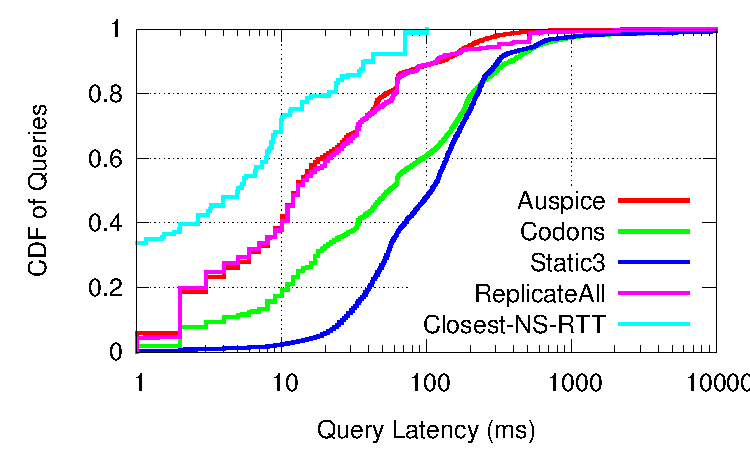
\includegraphics[scale=0.45]{graph/system-exp/cdf-comparison.pdf}}
\subfigure[Median lookup latencies for names.]{\label{fig:namesquerymediancdf}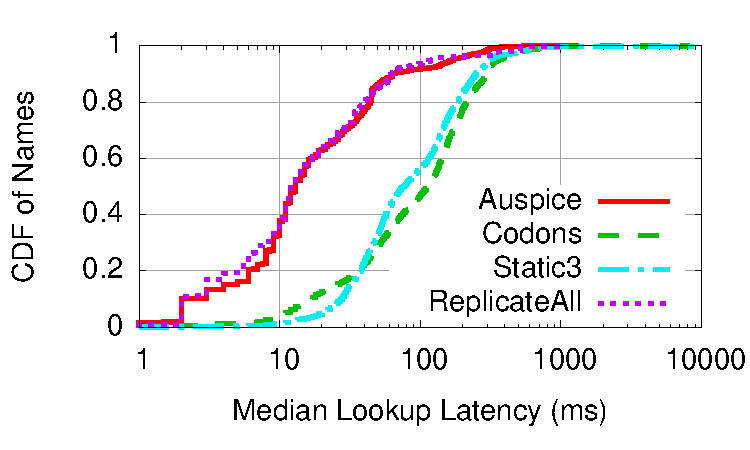
\includegraphics[scale=0.45]{graph/system-exp/cdf-names-median.pdf}}
\subfigure[Update cost of names.]{\label{fig:updatebw}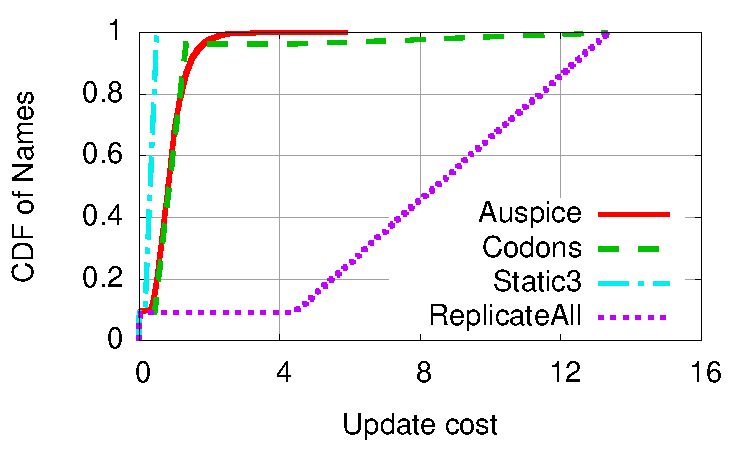
\includegraphics[scale=0.45]{graph/system-exp/cdf-update-cost.pdf}}
\caption{\auspice's lookup latency is nearly equal to \replicateall, yet its median update cost is 10$\times$ less. Locality-unaware schemes, \staticthree\ \& \codons, result in up to 6$\times$ higher median latencies than \auspice.}
\label{fig:lookupupdate}
\end{figure*}


% mobile

We present an evaluation of \auspice\ based on a PlanetLab deployment, cluster-based emulation, and a large scale experiments using our custom simulator. Further, we compare \auspice's performance to today's managed DNS services. 

\begin{itemize}
\item
Locality-aware placement helps \auspice\ achieves nearly 5$\times$ lower latency than a DHT-based replication scheme.
\item
\auspice\ reduces updates costs by nearly an order of magnitude over a replicate-everywhere strategy in a live deployment and yet achieves nearly identical query latencies.
\item
\auspice's load-aware design consistently achieves up to 2 $\times$ lower latencies under a wide range of load scenarios.
\item
With an equal number of name server deployments, \auspice\ achieves comparable DNS lookup latencies to a leading managed DNS provider today, and an DNS update latency which is nearly 2 seconds smaller.
\end{itemize}



%Our evaluation has three main findings. 
%(1) We show that \auspice's strategy of  replicating name records in a locality-aware manner based on read-to-write ratio gives significantly better performance over  locality-unaware replication schemes, including replication schemes implemented over a DHT.
%(2) We show that a global name service can leverage weaker consistency semantics for name records that are updated rarely, including domain names in today's Internet, to significantly reduce user-perceived latency as well as reduce load on the system.
%(3) Mid-session mobility conclusion.


%In this section, we describe our experimental evaluation of \auspice\ on PlanetLab as well as through  trace-driven simulations based on realistic workloads. %We begin with a description of the datasets used to generate workloads.
%Our evaluation has three main goals. 
%First, is to quantify the performance gap between optimal service placement and heuristic service placement strategies in \auspice.
%Second, is to evaluate performance of service placement  schemes in a scenario with high update rates, e.g. a name service for a near future Internet consisting of highly mobile users. 
%Third, is to answer whether service placement decisions considering
%the geo-distribution of users requests improves performance over
%schemes that are agnostic to geo-distribution of users, e.g. \codons. 

%\subsection{Evaluation goals}
%We present an evaluation of the service placement algorithms implemented in \auspice\ on the service workload datasets in Section \ref{sec:datasets}.



\subsection{Replica placement schemes comparison}


In this section, we compare the locality and load-aware replica placement scheme implemented in \auspice\ against alternate replica placement schemes. In line with our goal of designing a name resolution service for mobile hosts in the Internet, we focus on scenarios where a high fraction of name records belong to mobile hosts, with each device updating its network address at high frequency. We conduct experiments with the \auspice\ system comparing replica placement schemes on PlanetLab. For larger scale experiments infeasible on PlanetLab, we present results from a simulator that implements the same replica placement schemes.

%Overall conclusion: Locality-aware scheme does provide a lower latency for a comparable number of replicas, and a comparable load-balance.  (i). \codons's replication achieves poor latency across names. (ii) Naive strategies such as \staticthree\ and \replicateall\ perform worse than schemes that make a controlled number of replicas based on the read to write ratio. (iii) Making controlled number of replicas  based on read-to-write ratio in a locality aware manner provides up to 4$\times$ benefits in terms of latency if those replicas are created randomly.



\subsubsection{Schemes compared}


%\textbf{\locaware} refers to the locality-aware replica placement scheme implemented in \auspice. 

%
\textbf{\codons} is a DNS design implemented on top of Pastry DHT. \codons\ replicates a name record based on its popularity ranking, with more popular name records replicated at greater number of  locations.  The location of replicas is decided by consistent hashing. Our \codons\ implementation retains these features. However, we do not implement multi-hop DHT routing used in \codons. Each request is directly sent to the replica  that would have received this request if Pastry DHT routing were followed.
We achieve this behavior by copying the Pastry routing table of every node at all other nodes and simulating multi-hop routing locally.
Therefore, our latency numbers are a conservative estimate of the latency in \codons. 

\textbf{\staticthree} replicates each name record at three locations that are chosen randomly. \textbf{\replicateall} replicates all name records at all locations. 

\textbf{\opt} uses our optimization formulation (given in Appendix \ref{sec:optimal}) to minimize the total latency including network and server latency.  \opt\ serves as a benchmark for comparison and is implemented only in our simulator. \opt\ is an impractical scheme because solving the optimization problem for billions for name records is well beyond the scope of modern day LP solvers.

%At Internet scale, \opt\ is impractical because of the challenges in solving the optimization problem for billions of name records. 



\subsubsection{Workload}

Our workload consists of lookup requests for name records and updates to them from clients distributed across the globe. In this workload, name records are of two types: \emph{service names} and \emph{device names}. Service names correspond to today's DNS name records, which belong to immobile hosts. Device names correspond to name records for mobile hosts.

Our workload for service names is generated based on traffic statistics for websites reported in Alexa Web Information Service \cite{alexa} (AWIS) dataset. This dataset reports the relative popularity of each website and the geo-distribution of website's popularity at city-level granularity. 
Across different experiments, we generate a workload based on top-1000 and top-10000 most popular websites in this dataset. Today's DNS name records change slowly. Therefore, the number of updates to name records of a service names are less than 1\% of the number of lookup queries in the workload.

%To generate a workload for mobile names, 
%we assume that 

The device names workload exhibits high update rates and a strong geographic locality. The number of updates for a device name are 2-3 orders of magnitude higher than that of a service name. The geo-distribution of requests is as follows: 90\% of requests for a device name originate from 0-5\% of local name servers which are geographically close to each other; remaining 10\% of requests are generated from 5\% local name servers located farther away.

%. \% of requests originate from 0-5\% of local name servers . 

%To generate this workload, every local name server is assumed has an equal number of mobile hosts that send network address updates for their respective device names. 
%Thus,  updates for a mobile name are sent from a single local name server. 
% 90\% of requests for this mobile name are generated from this local name server and up to three  local name servers close to it;  remaining 10\% of queries are generated from 5 local name servers located farther away.

\eat{
The workload for mobile names has two key features. 
First, updates rates for mobile names are much higher than regular names. 
This is because the mobile host that owns a mobile name rapidly changes the set of networks it is connected to. 
Second, requests for a mobile name show strong geo-locality patterns. This is due to several reasons.
Updates for mobile names will originate from the mobile device itself, whose mobility will be contained in a small geographic region for most hosts.
A mobile name will be queried by web services to push updates to the mobile device. Today's web services are geo-replicated to position themselves closer to end-users. Most likely, the closest service replica will query for the mobile name, giving rise to geo-locality.
Another source of a mobile name's queries is communication between two mobile hosts, e.g., a user's friends contacting the user's mobile device to send messages. 
We expect these queries to come from a user's contacts list. Since most of a user's contacts are expected to be within  the same country, these  queries will exhibit strong geo-locality patterns as well.
}



\subsubsection{PlanetLab deployment}

%\begin{minipage}[b]{0.33\linewidth}
%\centering
%\includegraphics[scale=0.45]{newgraphs/pldata1.pdf}
%\caption{Dependence of swarm performance on server bandwidth, and peer arrival rate $\lambda$ for $S$ = 10MB and $\mu$ = 100KBps. Unit of $\lambda$ = sec$^{-1}$.}
%\label{fig:basic}\end{minipage}
%\hspace{0.45cm}

%   \subfigure[$\lambda = 0.45/sec$]{\label{fig:g1-time}\includegraphics[scale=0.34]{newgraphs/target-g1-time.pdf}}




%x	Auspice	Codons	Static3	ReplicateAll	
%Overall-Fairness	0.880849740715	0.983016103853	0.969862385826	0.944348480834	
%Update-Recvd-Fairness	0.923389058562	0.994508958801	0.987580628539	0.943487244312	
%Query-Fairness	0.633390113602	0.780041293236	0.903677640012	0.496513039982	




%
%\begin{figure}
%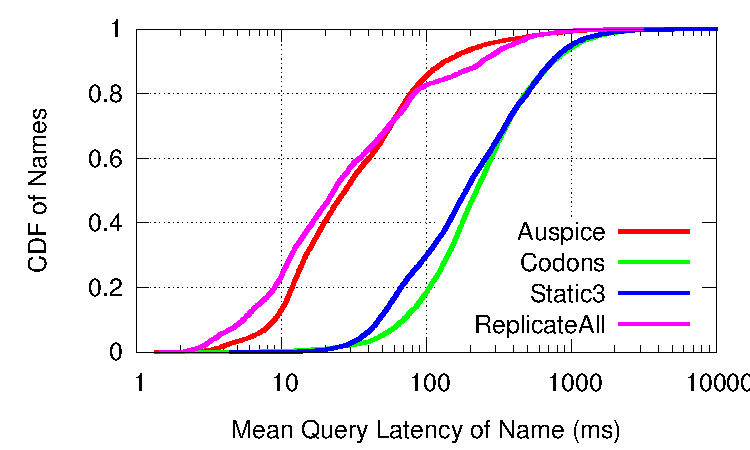
\includegraphics[scale=0.45]{graph/system-exp/cdf-names-mean.pdf}
%\caption{CDF of mean latency of queries for all names.}
%\label{fig:namesquerymeancdf}
%\end{figure}
%
%
%\begin{figure}
%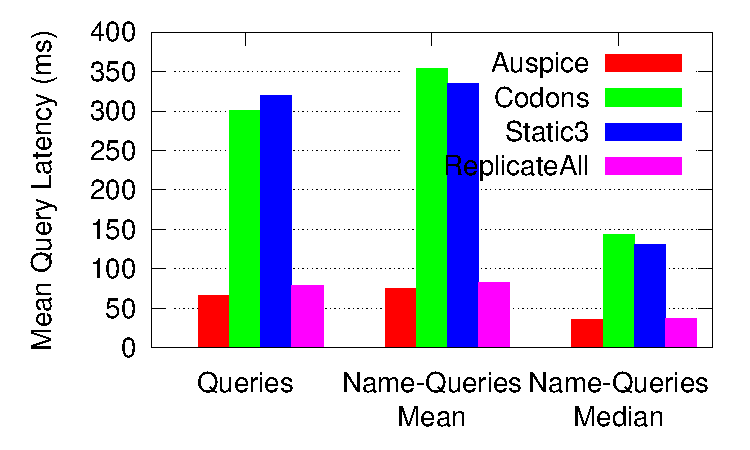
\includegraphics[scale=0.45]{graph/system-exp/mean-latencies.pdf}
%\caption{(1) Mean latency of all queries, (2) Mean of mean latencies of queries for all names, (3) Mean of median latencies of queries for all names}
%\label{fig:meanlatency}
%\end{figure}

%\begin{figure}
%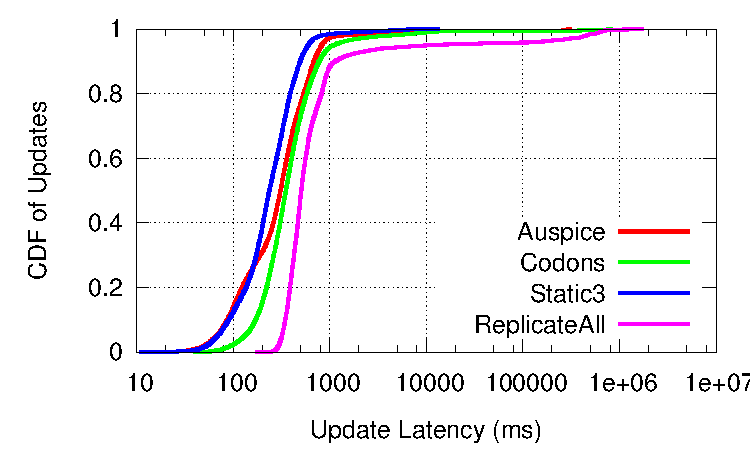
\includegraphics[scale=0.45]{graph/system-exp/cdf-comparison-update.pdf}
%\caption{CDF of  latency of all updates.}
%\label{fig:udpates}
%\end{figure}



%\begin{figure}
%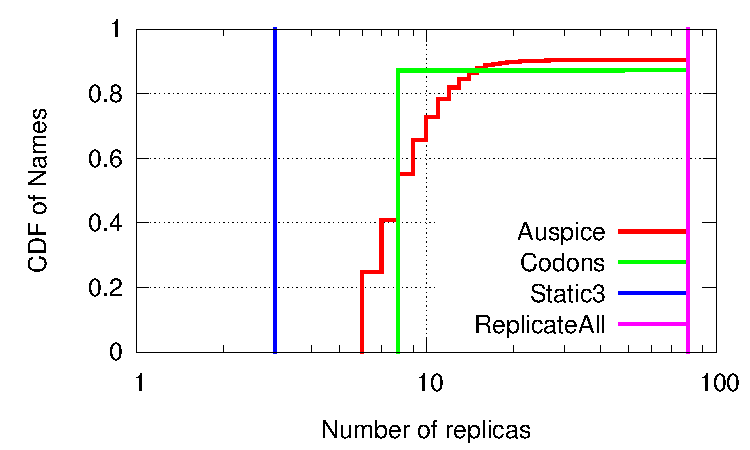
\includegraphics[scale=0.45]{graph/system-exp/cdf-replica-count.pdf}
%\caption{Distribution of the number of replicas for names.}
%\label{fig:cdf-replica}
%\end{figure}






%
%\begin{figure}
%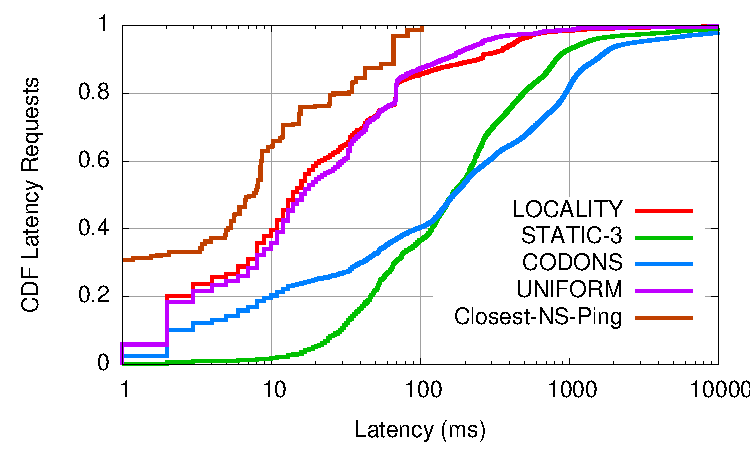
\includegraphics[scale=0.45]{graph/system-exp/high-cdf-comparison.pdf}
%\caption{High load, CDF of latency of all queries. NEW: load balancing, LNS votes for closest NS depending on (network + server) latency. $\alpha$ selected assuming server capacity = 200 req / sec.}
%\label{fig:highquerylatencycdf}
%\end{figure}
%
%\begin{figure}
%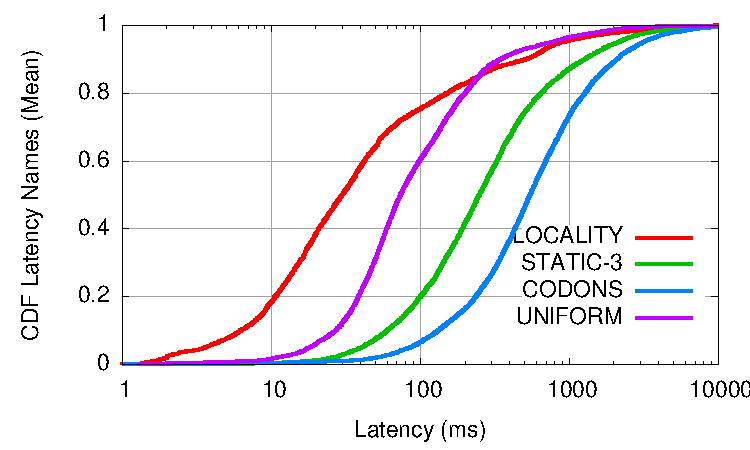
\includegraphics[scale=0.45]{graph/system-exp/high-cdf-names-mean.pdf}
%\caption{High load, CDF of mean latency of queries for all names.}
%\label{fig:highnamesquerymeancdf}
%\end{figure}
%
%\begin{figure}
%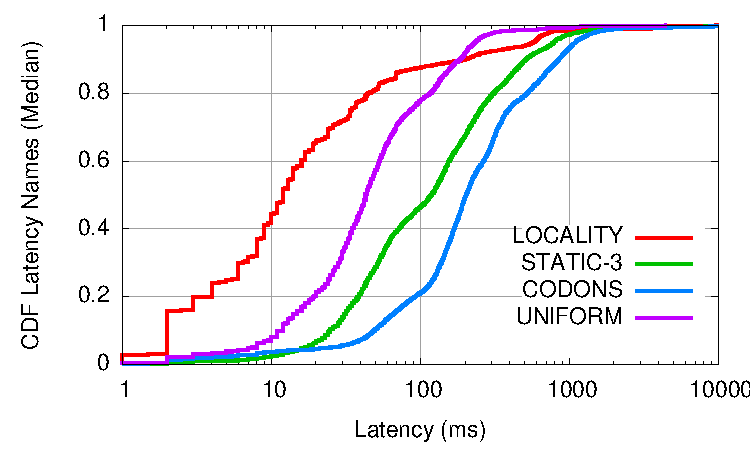
\includegraphics[scale=0.45]{graph/system-exp/high-cdf-names-median.pdf}
%\caption{High load, CDF of median latency of queries for all names.}
%\label{fig:highnamesquerymediancdf}
%\end{figure}



%
%\begin{figure}
%\vspace{1in}
%%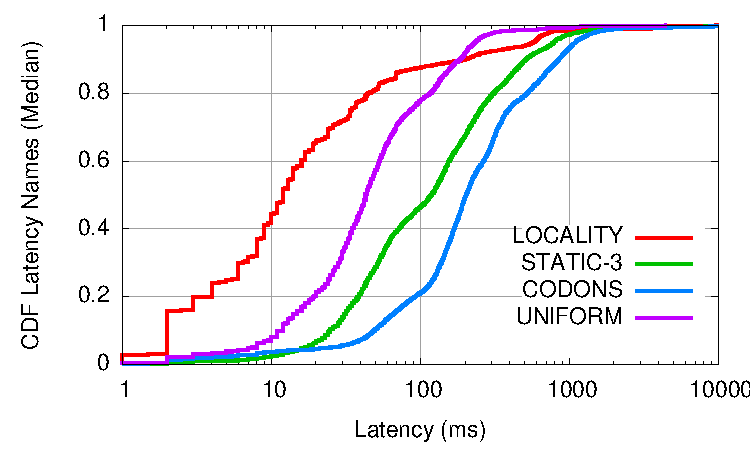
\includegraphics[scale=0.45]{graph/system-exp/high-cdf-names-median.pdf}
%\caption{Latency of \uniform\ as number of replicas is increased compared to the latency of \locaware\ in high load experiments. This graph shows that \uniform\ is not able to outperform \locaware\  even when given the freedom to create unbounded number of replicas. For uniform, increasing the number of replicas starts to increase server latency due to the cost of keeping number of replicas updated.}
%\label{fig:uniform}
%\end{figure}


%\begin{figure}
%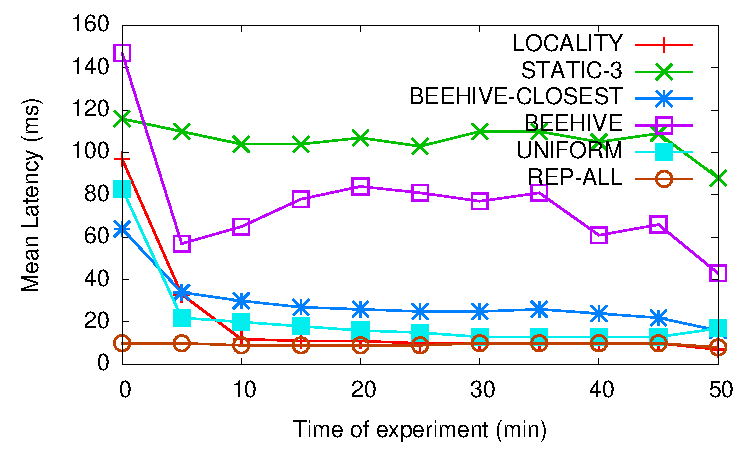
\includegraphics[scale=0.45]{graph/system-exp/timeline-median.pdf}
%\caption{Latency of queries over time. Each point shows the median latency of queries that arrived in the next five minutes.}
%\label{fig:medianlatencytime}
%\end{figure}



Our PlanetLab deployment was done on 160 nodes, 80 nodes running the name server module and 80 nodes running the local name server module. Clients are co-located on the nodes running the local name server module. If PlanetLab nodes are selected randomly, most nodes chosen are either in North America or in Europe.  We use a simple heuristic to select PlanetLab nodes spread across the world. 
For each user-group, the geographically closest local name server location is chosen as its proxy location, e.g., 80 PlanetLab locations  act as a proxy for nearly 15000 cities in the AWIS dataset.


Our workload consists of 4 million lookup requests and 2 million update  requests for  1000 service names and 10000 device names.  Lookup requests are divided equally between service and device names, but almost all updates belong to device names, and only 500 updates are for service names. The requests in the workload are sent over a duration of 30 minutes.


We have configured all schemes to ensure a fair comparison of their replication algorithms. The replication parameter for \locaware\ is calculated assuming each PlanetLab node can serve at least 300 requests / sec with a negligible delay. We have chosen the server capacity somewhat conservatively due to heterogeneity in PlanetLab nodes and because each node is shared among multiple users. 
For the \codons\ scheme, the Zipf exponent is set to $0.63$ calculated based on our workload, and the average hop-count is set to 0.55 which ensures that \codons\ creates nearly the same number of replicas in aggregate as \locaware\ and \uniform.  All schemes use the name server latency estimation implemented in \auspice\  to select the closest replica based on network latency and server latency. An exception is \codons, in which replica selection depends on DHT routing. 

%Figure \ref{fig:cdf-replica} shows the distribution of the number of replicas created by every scheme. 

%\eat{Locality-aware replica placement is configured by setting the replication parameter $\alpha$ = 0.2. This value of $\alpha$ implies that, in this experiment,  a name server will receive 15 requests / sec  on average (as per Equation 14), which clearly is less than the actual capacity of server. Thus we have made a conservative choice in selecting the replication parameter.  A higher alpha value will create more replicas and will likely lower the query latency. The parameters for \codons\ are set to the same values as described in their paper \cite{codons}.}

%We compare replication schemes on four metrics: latency of name record queries (Figure \ref{fig:querylatencycdf}, Figure \ref{fig:namesquerymeancdf}, Figure \ref{fig:namesquerymediancdf}, Figure \ref{fig:meanlatency}),  bandwidth needed to keep name record replicas consistent (Figure \ref{fig:updatebw}), latency of propagating address updates (Figure \ref{fig:udpates}), and a fairness metric to evaluate load balancing property (Figure \ref{fig:fairness-system}). 



%We first compare schemes based on their lookup latencies and update costs 

%We first evaluate schemes on their lookup latency and their update costs Figure \ref{fig:lookupupdate}. Figure \ref{fig:querylatencycdf} shows the CDF of latency of queries of every scheme. A limitation of Figure \ref{fig:querylatencycdf} is that the distribution is biased towards the more popular names in the workload. We expect a global name service to provide low latencies for all names and not just the most popular names. So, we compare the CDF of median  latency of queries for each name in the workload in Figure\ref{fig:namesquerymediancdf}. To evaluate the steady-state performance of all schemes, the latency of initial 25\% of queries are not included in these graphs. 




A locality-aware placement helps \auspice\ to achieve nearly the same lookup latencies as \replicateall, with one-tenth smaller median update cost for a name record than \replicateall. In other words, \auspice\ can match a scheme that uses nearly 10$\times$ as many resources. The \replicateall\ scheme uses 10$\times$ the upload and download bandwidth to propagate updates; it also uses 10$\times$ more server resources to process update messages. A locality-aware design makes efficient use of resources and in scenarios where resources are scarce, it can achieve better performance as well.

%\replicateall\ also adds to server load since every name server must process updates to all name records. In this experiment, PlanetLab nodes indeed have enough server capacity to handle updates to all name records, and therefore server load induced latency is negligible. In a scenario where compute resources are a bottleneck, \replicateall\ could result in poor query latency as is creates due to high server load. 

Locality-unaware schemes such as \staticthree\ and \codons\ cause high latencies. \staticthree\ has a very weak geo-locality of replicas as it chooses three replica locations randomly. While \codons\ create nearly the same total number of replicas as \auspice,  it  answers queries from a replica selected using DHT routing. In many cases, the latency to the selected replica  is higher than the latency to the closest replica for a name record. All other schemes, including \staticthree\ always choose to the closest replica for a name record and hence achieve lower latencies than \codons.  \codons\ replicates 11.2\%   most popular names at all locations. Queries for these names indeed go to the closest replica and achieve low latencies; queries for remaining 88.2\% of names incur high latencies. \codons's design achieves good load balancing under heavy load scenario. In a moderate load scenario, this design results in poor latencies.




\begin{figure}
\centering
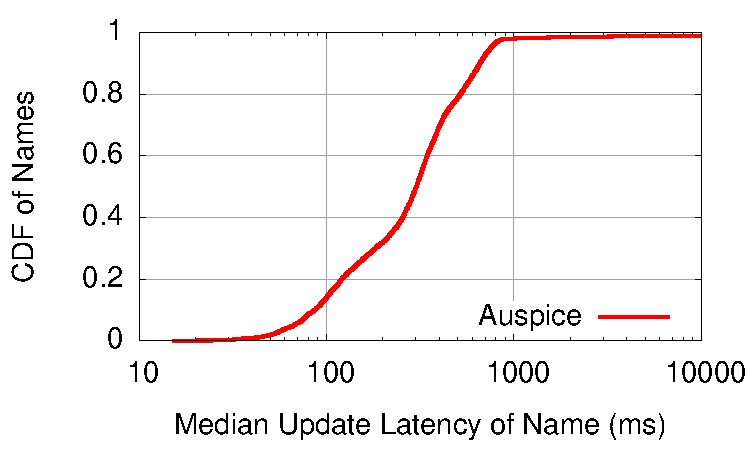
\includegraphics[scale=0.45]{graph/system-exp/cdf-names-median-update.pdf}
\caption{Address update latency of \auspice\ is comparable to other schemes. The high latencies for \replicateall\ are because of insufficient upload capacity on PlanetLab nodes.}
\label{fig:udpates}
\end{figure}

\begin{table}[t]
\centering
\begin{tabular}{ l | c | c}
\hline
Scheme & Update-fairness & Lookup-fairness\\
\hline
\auspice\ & 0.92 & 0.63 \\ 
\hline
\codons\ & 0.99 & 0.74 \\
\hline
\staticthree\ & 0.98 & 0.84 \\
\hline
\replicateall\ & 0.94 & 0.49 \\
\hline
\end{tabular}
\caption{\auspice\ ensures an even distribution of update load among name servers; its lookup fairness is moderately lower due to its locality-aware placement and redirection.}
\label{tab:top10web}
\end{table}


\begin{figure}
\centering
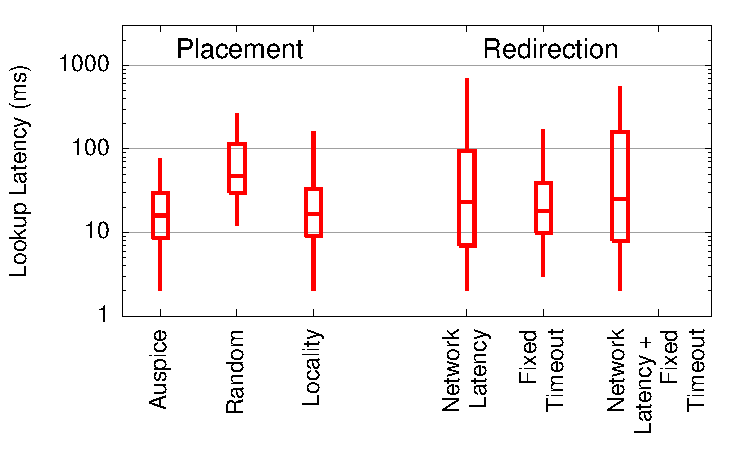
\includegraphics[scale=0.45]{graph/system-exp/mb-stats.pdf}
\caption{Micro benchmarks of \auspice\  show that locality-awareness in the placement phase and load-balancing in the redirection phase are important to achieve good performance.}
\label{fig:micro}
\end{figure}


Address update latency is an important metric for a global naming service . \auspice's address update latencies are of a few hundred milliseconds, and are comparable to that of \staticthree\ and \codons (Figure \ref{fig:udpates}). The \replicateall\ scheme has higher update latencies as it propagates updates to a much greater number of replicas. In our implementation,   an address update is first sent to the Paxos co-ordinator for this name record,  which waits for a confirmation from a majority of replicas, and then replies to the client that the update is complete.  Since the Paxos co-ordinator is chosen randomly among replicas, update latency for all schemes is roughly equal to twice of the round-trip latency between a pair of randomly chosen PlanetLab nodes. This explains why typical update latencies are of a few hundred milliseconds.


The \replicateall\ scheme has median update latencies of 100-1000 seconds for 15\% of names. This is because updates for these names are handled by nodes whose upload capacity is less than that required by \replicateall\ scheme. As a result, updates get queued at name sever and completed updates reflect in the form of high update latencies. 


Do the latency benefits of  a locality-aware placement come at the cost of creating load imbalance at name servers, and how does the load balancing achieved by \locaware\ compare to other schemes? We evaluate the load balancing property in terms of a fairness score \cite{jain-fairness}. The fairness-score is calculated over the number of lookups (updates) received at every name server, and is termed \emph{lookup-fairness} (\emph{update-fairness}). 

All schemes, including \auspice, achieve a  high update-fairness score above ($>$ 0.90), suggesting that update load is balanced evenly across name servers. 
\auspice\ selects replicas based on locality as well as randomly which helps in an even distribution of update load among name servers. 
All schemes achieve a lower score on lookup-fairness ranging between 0.49 (for \replicateall) and 0.84 (for \staticthree). \auspice's achieves a lower lookup-fairness than locality-unaware schemes \staticthree\ and \codons\, but better lookup-fairness of locality-unaware schemes is far outweighed by their poor lookup latencies.

%\locaware\ and \uniform\ have comparable query-fairness suggesting that creating replicas in a locality-aware manner does not significantly hurt the load balancing property. \codons's query-fairness is 33\% higher than that of \locaware, but its better query-fairness is far outweighed by its worse query latency (Figure \ref{fig:namesquerymediancdf}).
%Overall fairness is high despite a lower query-fairness because the number of update messages outnumber queries by at least 3 to 1 for every scheme except static-3.



%For this reason, these nodes could not could not complete all address updates during the experiment. 
%resulting in incorrect network addresses returned to clients. 


%We performed micro-benchmarks  with \auspice\ on PlanetLab to study how each component of its design affects its performance. Each experiments measures \auspice's performance by changing either its resolver placement algorithm or its redirection strategy. Each experiment was repeated three times on three different days and median value is reported. 

Our next experiment presents micro benchmarks for \auspice\ and shows that both its locality-aware placement and its load-aware redirection scheme help to achieve lower latencies. Our micro benchmarks evaluate variants of \auspice's design, and we group our results into two categories, placement and redirection, depending on which aspect of \auspice's design is varied. Figure \ref{fig:micro}  presents our results, and shows mean of the distribution of median latencies of lookups for each name record.

We evaluate two variants of \auspice's placement algorithm, \uniform\ and \locaware. These scheme choose the same number of replicas as \auspice, but \uniform\ chooses all replicas randomly to maximize load balance, and  \locaware\ chooses all replicas based on demand locations.  \auspice\ achieves nearly 4$\times$ lower latencies than \uniform, while the \locaware\ scheme achieves only 20$\%$ higher latencies than \auspice. 
The benefit of a locality-aware placement over a random placement (\uniform) depends on the number of replicas. 
Name records that have a high read-to-write ratio, and are replicated at a large fraction of locations, benefit little from a locality-aware placement. 
Names with a small read-to-write ratio, which are replicated at a small number of locations, achieve a lower latency with a locality-aware placement than a random placement.  In this experiment,  80\% of names are replicated at less than 12 locations, and therefore a locality-aware placement helps. 

%These 80\% of names account for less than 50\% of requests. This explains why the gains of \locaware\ over \uniform\ are greater in  Figure 4 and Figure 5 which compares latency across names, than in Figure 3 which compares latency across requests.


\auspice's redirection strategy has two main components: adaptive timeout and name server latency estimation based on server load and network latency (called load-balancing in short). We evaluate three \auspice\ variants that disable one or both of these features. Instead of using adaptive timeout, we use a fixed timeout value of 150ms which is equal to 95th percentile lookup latency \auspice\ in Figure \ref{fig:querylatencycdf}. Figure \ref{fig:micro} shows that disabling the load-balancing component increases the query latency by nearly 6$\times$. Load-balacing helps identify a few PlanetLab server that are experiencing high load which significantly reduces mean query latencies. A fixed timeout of 150 ms gives higher latencies than an adaptive timeout values. While it is possible to choose a fixed timeout value more carefully, adaptive timeout provides good performance and does not require parameter tuning.








%\locaware\ achieves nearly the same lookup latency as \replicateall\  but 

%\locaware\   and \replicateall\ both achieve the least query latency among all schemes, 
%but \replicateall\ scheme consumes nearly 9$\times$ more download bandwidth at a typical node than \locaware\ to keep name records consistent (Figure \ref{fig:updatebw}).
%\replicateall\ consumes an equally high upload bandwidth at a typical node to push address updates to all other name servers  (graph omitted for brevity). 
%

%To validate this claim, we performed a experiment on a cluster environment with gigabit-capacity network links. The aggregate update rate was nearly 3$\times$ higher than in the PlanetLab experiments. In this case, \replicateall\ scheme resulted in a worse query latency than  \staticthree\ and \locaware.





%\locaware\ creates the nearly same number of replicas as \uniform\ for every name (Figure \ref{fig:cdf-replica}), but it creates them close to the pockets of demand resulting in a lower query latency.


%The benefit of locality-aware placement is greater for mobile names than for regular names.

%Regular names have a high ratio of (read rate) / (write rate), hence both \uniform\ and \locaware\ create a large number of replicas of regular names. 
%For this reason, locality-aware placement of replicas provides less benefits to \locaware\ over \uniform\ for queries belonging to regular names, that constitute 86\% of all queries.
%The (read rate) / (write rate) ratio of mobile names is less than 1, hence only one active replica is created for mobile names. The \locaware\ scheme achieves a lower query latency than \uniform\ by placing an active replica in a locality-aware manner. Since 89\% of names are mobile names, this also explains why \locaware\ shows high gains over \uniform\ when CDFs across names are compared.


%\replicateall\ strategy is wasteful of network and server resources, and \locaware\ scheme achieves the same query latency while using much less resources.  



% comparison of locality and replicate all
%\eat{The \replicateall\ scheme does achieve a lower latency than \locaware\ but \replicateall\ creates 7.15$\times$ more replicas than \locaware\ or \uniform\ in this experiment. \replicateall\ is not a practical scheme for a global name service because each node must handle all updates. The aggregate update rate of a global name service  will exceed the capacity of a single node which will result in poor performance. To validate this claim, we performed a experiment on a cluster environment with an aggregate update rate of 2750 req/sec in which \replicateall\ scheme resulted in a worse query latency than  \staticthree\ and \locaware.}




%\subsubsection{Throughput under high load}

%In this experiment, we have shown that replicating name records in a locality-aware manner based on the read-to-write ratio gives the best performance. The experiments with our \auspice\ prototype were conducted on a  smaller scale workload than a global name service is expected to handle and and our server deployment was restricted by the number of reliable geo-distributed PlanetLab servers we could obtain. Therefore, we next present experiments from our simulator that that compares replication schemes for a larger server deployment and workload sizes.

\subsubsection{Simulator}



One question to discuss. How do replication schemes compare at low-load (0-10\%), moderate-load (50\%)and high-load (90\%) scenarios. In the system experiment, the locality-benefits of \locaware\ outweigh the load-balancing benefits of \uniform\ and \codons. When this load increases, is there a regime where load balancing benefits of \uniform\ and \codons\ enable them to outperform a locality-aware replication scheme? 


\subsection{Comparison to managed DNS services}


%\subsection{Benefits of high TTL}

%\begin{figure}
%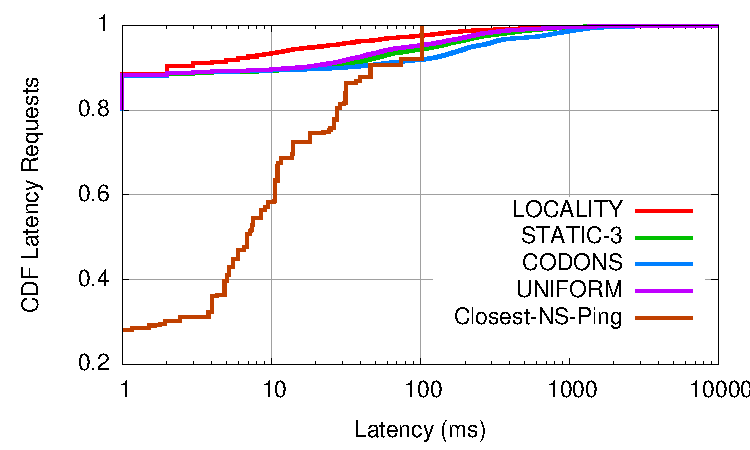
\includegraphics[scale=0.45]{graph/system-exp/ttl-cdf-comparison.pdf}
%\caption{High TTL, high load, CDF of latency of all queries. TTL are set comparable to the write rates of regular names. TTL are set comparable to be write rates of regular names.}
%\label{fig:ttlquerycdf}
%\end{figure}
%\begin{figure}
%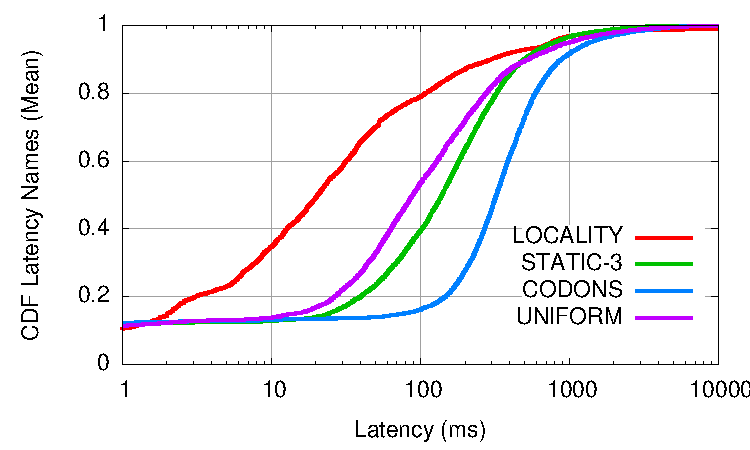
\includegraphics[scale=0.45]{graph/system-exp/ttl-cdf-names-mean.pdf}
%\caption{High TTL, high load, CDF of mean latency of queries for all names.}
%\label{fig:ttlnamesmean}
%\end{figure}
%\begin{figure}
%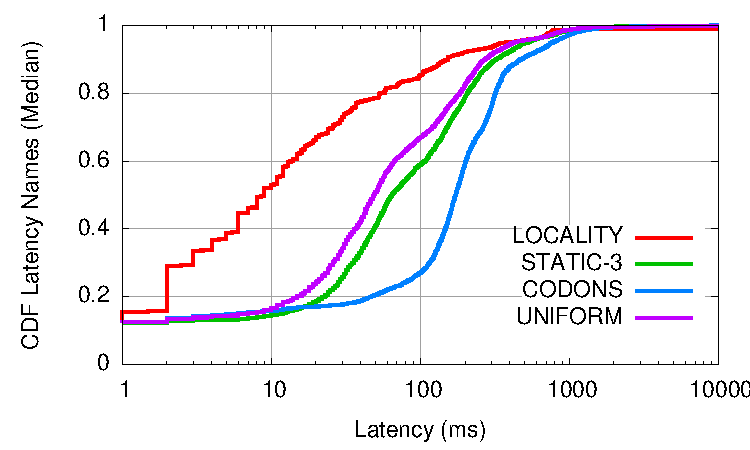
\includegraphics[scale=0.45]{graph/system-exp/ttl-cdf-names-median.pdf}
%\caption{High TTLs, high load, CDF of median latency of queries for all names.}
%\label{fig:ttlnamesmedian}
%\end{figure}

%High TTLs can significantly lower the latency for regular names queries. 



%\begin{figure}
%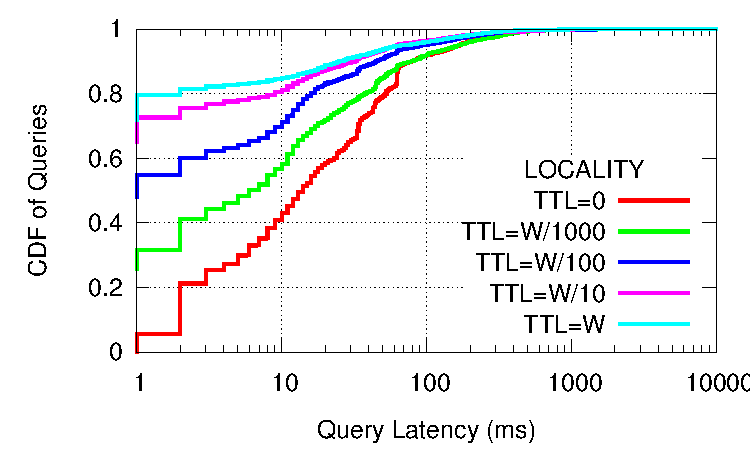
\includegraphics[scale=0.45]{graph/system-exp/ttl-cdf.pdf}
%\caption{W = average interval between change of network address for regular names. A TTL-value equal to W/10 provides considerable reduction in latency over a TTL-value of zero or the using a TTL-value 100-1000$\times$ smaller than W.}
%\label{fig:ttlvary}
%\end{figure}

%\begin{figure}
%\vspace{1.5in}
%\caption{This graph shows the latency CDF across names for \locaware\ when TTLs are set to 0.01\%, 0.1\%, 1.0\%, 10.0\% of write rate for mobile names. High TTLs reduce the load on the system resulting in improved latency for mobile names as well.}
%\label{fig:ttlvarynames}
%\end{figure}



%(2) Codons scheme performs well for names it replicates every where, for other names in most cases it performance is worse than Static-3 which replicates names. Focus on load balancing results in poor latencies. If we compare latency across names, its performance is the worst.

%(3) The difference between Uniform and Locality shows the value of placing replicas in a locality-aware manner.

%(4) Compare the number of replicas: locality creates less replicas than beehive and  uniform scheme. 

%
%
%Write performance: 
%
%Write latencies are comparable. 




%\subsubsection{Simulator}


%\subsection{Comparison to DNS}
%This section compares \auspice\ to today's DNS. Through distributed measurements on PlanetLab testbed.


\subsection{Mid-session mobility}

